% TODO: I need a figure with some psychometric showing good performance. 
% Some cool additional analysis that would be nice to include if I have time. 
%TODO: How long does it take to learn the categorization once the initial exemplars are learned? 
%TODO: How long does it take to learn to switch after you are able to categorize? 
%TODO: How long does it take to learn the second category after you are able to learn the first? 

% Figures in this chapter
\newcommand{\Task}{1} \newcommand{\TaskDiagram}{\Task A}
\newcommand{\TaskTrials}{\Task B} \newcommand{\TaskSounds}{\Task C}

\newcommand{\Training}{2} \newcommand{\TrainingSessions}{\Training A}
\newcommand{\TrainingTrials}{\Training B}

\newcommand{\amod}{3} \newcommand{\amodPsychometrics}{\Amod A, B, D, E}
\newcommand{\amodCorrect}{\Amod C, F}

\newcommand{\SingleSound}{4} \newcommand{\SinglePsy}{\SingleSound A, C}
\newcommand{\SingleSum}{\SingleSound B, D}
\newcommand{\SingleFreqP}{\SingleSound A}
\newcommand{\SingleFreqS}{\SingleSound B} \newcommand{\SingleAMP}{\SingleSound
C} \newcommand{\SingleAMS}{\SingleSound D}

\chapter{A behavioral task for evaluating the cortical and subcortical
contributions to sound feature discrimination}

\section{Introduction}
% We found that corticostriatal and thalamostriatal pathways send different
% information about certain sound features to the striatum. 
% DONE: Chapter number
In \ch{\Thstr}, we found that the thalamostriatal and corticostriatal
pathways send complementary information to the striatum about some features of
sound. 
%
While both pathways conveyed frequency information to the striatum with similar
fidelity, corticostriatal neurons better represented the rate of temporal
amplitude modulations in their overall spiking rate.
%
The spiking rate of thalamostriatal neurons more closely followed rapid
variations in stimulus amplitude, but the total number of spikes during the
stimulus was less indicative of the modulation rate.
% What is the significance of this difference? 
% DONE: Chapter number
While our earlier experiments in \ch{\Musc} strongly suggested a role for the
striatal target region of these projections in sound-guided behavior, the
relative contribution of these parallel pathways to behavior is unclear. 
%

% Some inactivation studies show that AM discrimination suffers after cortical
% lesions.
Lesion studies have suggested that discrimination of fast AM rates suffers
following removal of auditory cortex \citep{Deutscher2006}.
%
In contrast, sound frequency discrimination behavior has been shown to persist
after extensive lesions of AC \citep{Gimenez2015}.
%
% DONE: Phrase as either/or cortical/subcortical?
We therefore hypothesized that the cortical representation of AM is necessary
for accurate AM discrimination, but that sound frequency discrimination can be
accomplished with auditory information from the subcortex alone. 

% Specific hypothesis and test
Specifically, we hypothesized that the effect of reversible AC inactivation
would be greater on AM discrimination than on frequency discrimination. 
%
To test this hypothesis, we designed and implemented a behavioral task that
permits evaluation of the effects of a single reversible inactivation on
discriminations of both sound features.
%
We performed bilateral reversible inactivations of AC in animals trained on
this task, and found that discrimination of both features was impaired. 
%
While the contribution of the thalamostriatal and corticostriatal pathways to
discrimination of these sound features is still not clear, this task provides a
method for comparing the effect of reversible chemical manipulations on
discriminations of diverse stimulus features. 


\section{Methods}

\subsection{Animal subjects}
% DONE: Number of mice
14 adult male wild-type mice (C57/BL6J) were used in this study. Mice had ad
libitum access to food, but water was restricted. Free water was provided on
days with no experimental sessions. All procedures were carried out in
accordance with National Institutes of Health standards and were approved by
the University of Oregon Institutional Animal Care and Use Committee.

\subsection{Behavioral task}
% DONE: Update methods for amod task
Behavioral data was collected using the taskontrol platform
(\url{www.github.com/sjara/taskontrol}) developed in our laboratory using the
Python programming language (\url{www.python.org}).
%
Mice initiated each trial by poking their noses into the center port of a
three-port behavior chamber.
%
% DONE: We aren't making animals wait - check the paradigm After a silent delay
% of random duration (150-250 ms, uniformly distributed), a sound was presented
% for 500 ms.
%
The sound was either a narrow-band sound (chord), a single tone, or a
sinusoidally-amplitude-modulated white noise.
%
The decision to use chords or tones was chosen by the experimenter, and
thereafter during the behavior session the type of stimulus alternated between
cords/tones and AM sounds each trial (stimulus type was not randomized per
trial).
%
Animals were required to stay in the center port until the end of the sound and
then chose one of the two side ports for reward (2 $\mu$l of water) according
to a reward contingency that was specific to the type of sound.
%
For chords and tones, the reward contingency was: low frequency: go to left
port; high frequency: go to right port.
%
For amplitude-modulated noise, the reward contingency was: slow modulation
rate: go to left port; fast modulation rate: go to right port.
%
If animals withdrew before the end of the stimulus, the trial was aborted and
ignored in the analysis.
%
Chord stimuli were 12 simultaneous pure tones logarithmically spaced in the
range f/1.2 to 1.2f for a given center frequency f.
%
Within a behavioral session, we used 8 distinct center frequencies for chords
and tones, and 8 distinct modulation rates for AM sounds.
%
Each behavioral session lasted 60 to 90 minutes.

\subsection{Muscimol inactivation}
% TODO: Change to match muscimol protocol for amod study.  @internet
Bilateral craniotomies were performed under stereotactic surgery over the
posterior striatum (1.7 mm posterior to bregma, 3.55 mm lateral from midline)
of mice trained in the two-alternative choice sound discrimination task.
%
Headbars were implanted to allow for head-fixation.
%
Each craniotomy was protected with a plastic ring and filled with silicon elastomer (Sylgard 170, Dow Corning).
%
Animals were allowed to recover for at least 3 days before resuming behavioral training.
%
Following recovery, implanted animals were trained on the sound discrimination task until they reached their pre-surgery performance level before beginning muscimol inactivation.

For intracranial injection, we used glass pipettes (5 $\mu$l Disposable Micropipettes, VWR) pulled and trimmed to an inner diameter of 15-20 micrometers at the tip.
%
Animals were head-fixed and allowed to run on a wheel during the injection.
%
Craniotomies were exposed by removing the silicon elastomer covering, and a glass pipette filled with reagent (either muscimol or saline) was lowered into the brain to a depth of 3.1 mm from brain surface using a micromanipulator.
%
A volume of 45 nl of muscimol (0.25 mg ml$^{-1}$, final dose of 11.25 ng per hemisphere) was injected under air pressure in each hemisphere at a rate of 90 nl min$^{-1}$.  %
% Given the relationship between concentration and diffusion distance (from
% Fick's law) and previous reports of muscimol effects on neuronal activity
% \citep{Edeline2002}, we expect that by the first 10 minutes of the behavioral
% session, the effects of muscimol (50\% reduction in firing or more) will be
% confined to a volume smaller than 1 mm in diameter centered at the injection
% site. This volume matches well the extent of the posterior tail of the
% striatum (approx. 1 mm A-P, 0.6 mm M-L, 1.5 mm D-V) that receives auditory
% inputs \citep{Hunnicutt2016}.
%
The pipette was left in place for 60 seconds following the injection, then raised 0.5mm and left in place for another 60 seconds before being removed.
%
Injection in the second hemisphere was always completed within 10 minutes of the first injection.
%
The craniotomies were then protected with a new silicon elastomer cap, and the mouse was placed back into its home cage for 30 minutes before starting the behavior session.
%
After collection of 4 saline sessions and 4 muscimol sessions, 45 nl of fluorescent dye (DiI, Thermo Fisher Scientific) was injected at the same injection coordinates.
%
Animals were then perfused transcardially with 5\% paraformaldehyde, and brains were extracted and postfixed for 12-24 hours.
%
Brains were then sliced (100 um) and imaged to verify the location of fluorescent dye injection.  

\subsection{Analysis of behavioral data}

% DONE: Add stuff about the GLMER models here.
Psychometric curve fitting was performed via constrained maximum likelihood to estimate the parameters of a logistic sigmoid function (\url{http://psignifit.
%
sourceforge.net}). Statistical comparisons were performed using non-parametric statistical tests with no assumption of normality. 
%
Generalized linear mixed models were fit with the R programming language (\url{https://www.r-project.org/}) using the `lme4' package (\url{http://lme4.r-forge.r-project.org/}).  %TODO: I need to put the GLMER results in this document...


\section{Results}

% DONE: Table number
We found that this task was challenging to learn, but that animals could learn to perform it well if given sufficient training time.
%
We used a set of criteria defined in Table IV.1 to determine when mice were ready to advance to the next training step.
%
Animals first advanced through a series of behavioral stages designed to familiarize them with the behavior box and begin to teach them the rules of the task.
%
During the first stage, animals received a water reward after poking their nose
in any of the three ports in the box.
%
This stage allowed animals to learn that the behavior box is a good place to
be, and engaged their natural desire to explore to teach them that they are
able to control the environment and trigger changes by poking in the ports.
%
In the next stage, animals had to poke in the center port and then go to the
side ports to collect water.
%
This stage began to teach the animals that the center port is where you go to
trigger trials, and that going to a side port is how you collect reward.
%
During these first two stages, an auditory stimulus was played to the animals when they triggered a trial by sticking their nose in the center port.
%
After animals were acquainted with the box and the idea of poking to receive water, they began to learn the sound-action association.
%
% DONE: Mention sound above
During the next stage, animals triggered a trial by poking in the center port,
and then had to go to the right port to collect a reward if the AM rate of the
presented sound was fast, and to the left port if the AM rate was slow.
%
However, on this stage animals were guided towards forming the correct
association by letting them correct their choice if they first made a mistake.
%

After animals performed well on this stage, we started requiring animals to
make a correct choice on the first try.
%
% DONE: define the range
When they were performing well on this stage, we began presenting a range of AM
rates between the previously-trained fast and slow rates (usually 8 rates,
logarithmically-spaced between the slow and fast rate used in the initial training).
%
During this stage, animals had to learn the category boundary between the
``fast'' and ``slow'' rates.
%
Once they became proficient at this discrimination, animals had good knowledge
of the task structure and rules.
%
At this point, we began to train on two narrow-band stimuli (or pure tones for
some animals).
%
We then switched to a stage where we presented a range of frequencies, logarithmically-
spaced between the initial low and high frequency, and
trained animals until they had learned the boundary between ``high'' and
``low'' sound frequencies as well.
%
% DONE: At this point is ambiguous does it mean this or the next one?
After they had been trained to categorize first AM rate, and then frequency of sound,
we started to introduce the next level of task complexity.

During the next training stage, the type of sound presented when animals
triggered a trial switched between an AM noise and a narrow-band chord (or pure
tone) every other trial.
%
% DONE: Takes little time to do, which is a cool feature. Talk about that here. 
The sound-action association necessary to receive reward was the same as had
been previously learned for each sound.
%
We first introduced animals to the type of sound switching by presenting only
two examples of each sound type, but then moved on to presenting a range of AM
rates and sound frequencies.
%
% TODO: Number of sessions it took to learn the switching.
Animals took few sessions to learn to switch back and forth between the types 
of stimuli they were categorizing.
%%%%%%%%%%% Training structure table %%%%%%%%%%%%%%

%DONE: Last criterion to advance (to experiment ready)
After animals performed above 80\% correct on each discrimination for 3 consecutive training sessions, they were deemed ready for use in experiments. 

\begin{sidewaystable}
%\begin{table}
\resizebox{\textwidth}{!}{%
\begin{tabular}{lllll}
\textbf{Stage} & \textbf{Name}        & \textbf{Goal}                           & \textbf{Water delivery}       & \textbf{Criterion to advance}              \\
SD AM          & Sides Direct, AM     & Get animals to poke and collect water   & After center or side poke     & One session with 200 rewards               \\
D AM           & Direct, AM           & Trial initiation in center poke         & After center poke             & One session with 200 rewards               \\
NC AM          & On next correct, AM  & Discover correct association            & After correct/ed side poke    & One session with 500 rewards               \\
IC AM          & If correct, AM       & Enforce correct association             & After correct side poke       & Animal performs \textgreater{}80\% correct \\
P AM           & Psychometric, AM     & Categorize AM rate                      & After correct side poke       & Animal performs \textgreater{}80\% correct \\
IC F           & If correct, Freq     & Form association for frequency          & After correct side poke       & Animal performs \textgreater{}80\% correct \\
P F            & Psychometric, Freq   & Categorize sound frequency              & After correct side poke       & Animal performs \textgreater{}80\% correct \\
IC M           & If correct, Mixed    & Switch between sound types              & After correct side poke       & Animal performs \textgreater{}80\% correct \\
P M            & Psychometric, Mixed  & Categorize both sound types             & After correct side poke       & Animal performs \textgreater{}80\% correct \\
\end{tabular}}
%TODO: Table caption (just review it one more time before nobody ever sees it again). 
\caption{Stages of behavioral shaping.}{Animals progressed through 9 behavioral training stages during behavioral shaping.
%
Each stage was designed to teach the animal a new feature of the behavioral task.
%
Animals graduated to the next phase of training when they performed above a set criterion level.
%
Over the first three training stages, animals primarily learned about the behavioral box and the structure of the task.
%
After an initial session where a nose poke in any of the three ports would trigger water, animals next had to learn to trigger rewards by poking in the center and then collecting the reward at the side.
%
The sound-action association was trained over a series of three stages, where animals could initially correct a previous incorrect response and still get a reward.
%
After this stage, a correct response was required on the first poke.
%
Once animals were capable of performing the discrimination behavior with two prototype stimuli (well-separated in stimulus space), they were then tested with a range of stimuli logarithmically-spaced between the initial two prototypes, and were required to learn the category boundary.
%
Finally, once animals were capable of categorizing both AM rate and sound frequency, the sound triggered by every nose poke began to alternate between an AM noise stimulus and a tone every other trial.
%
Animals still had to perform the previously-learned categorization on each stimulus.}
\end{sidewaystable}
%\end{table}

%%%%%%%%%%%%%%%%%%%%%%%%%%%%%%%%%%%%%%%%%%%%%%%%%%%


\subsection{Animals can switch between discriminations of different stimulus
features every trial}

Despite the difficulty of learning this task, which was evident by the long
time required for animals to progress through all of the many training stages,
animals were able to achieve high levels of performance.
% TODO: I need a figure with some psychometric showing good performance. 

%%%%%%%%%%%%%%%%%%%%%%%% Figure Task %%%%%%%%%%%%%%%%%%%%%%%%%%%%%
\begin{figure}[hp] \begin{center}
	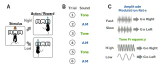
\includegraphics[width=6in]{figures/chapter4/figure_task} \end{center}
	\caption{A behavioral task for evaluating the effects of reversible
	inactivation on discrimination of different sound
	features.}{\textbf{(A)} Schematic of the two-alternative choice sound
	feature discrimination task. Mice initiated each trial by entering a
	center port and had to choose one of two side reward ports depending on
	the sound presented.
	%
\textbf{(B)} The type of sound presented was alternated every other trial. 
%
% DONE: Make sure all other figure captions have bold cap labels
\textbf{(C)} On trials when an AM noise stimulus was presented, mice had to
choose the right reward port if the modulation rate was fast and the left
reward port if the modulation rate was slow to be rewarded. On trials when a
narrow band chord was presented, mice were rewarded for picking the right port
if the sound frequency was high and the left port if the sound frequency was
low. 
%
}
\end{figure}
%%%%%%%%%%%%%%%%%%%%%%%%%%%%%%%%%%%%%%%%%%%%%%%%%%%%%%%%%%%%%%%%%%%%%

% DONE: I think this figure should come earlier. 
%%%%%%%%%%%%%%%%%%%%%%%% Figure Training Time %%%%%%%%%%%%%%%%%%%%%%%%%%%%%
\begin{figure}[hp] \begin{center}
	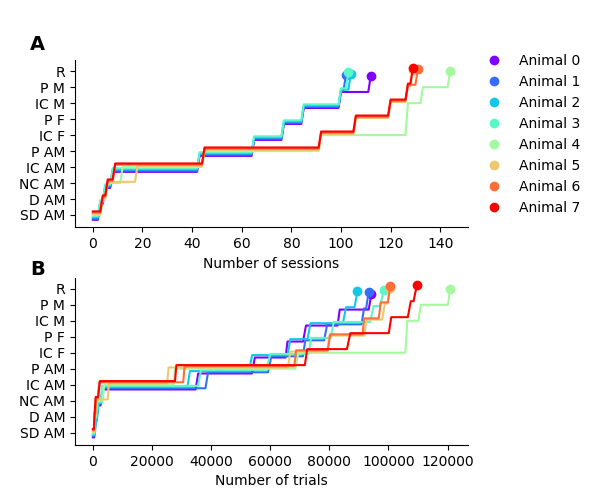
\includegraphics[width=6in]{figures/chapter4/figure_training}%
\end{center} \caption{Animals took about 4 months to learn the
task.}{\textbf{(A)} Animals progressed through 9 training steps over an average
of 119 behavioral training sessions before being ready for experiments (min:
102 sessions; max: 144 sessions). 
%
\textbf{(B)} Animals performed an average of 100,892 trials before being ready
for experiments (min: 89,527; max: 120,885). 
%
} \end{figure}
%%%%%%%%%%%%%%%%%%%%%%%%%%%%%%%%%%%%%%%%%%%%%%%%%%%%%%%%%%%%%%%%%%%%%

\subsection{Reversible inactivation of AC affects discrimination of both sound
frequency and AM rate} After animals had learned the task, we began performing
bilateral intracranial injections of either the GABA agonist muscimol, or a
saline control, 30 minutes before each behavioral sessions.
%
We alternated between muscimol and saline injections each day. 
%
Muscimol injection affected performance on both tone and AM trials, resulting
in both a flattening of the psychometric curve (\fig{\amodPsychometrics}) and a
reduction in overall performance (\fig{\amodCorrect}) for both animals tested. 
%
We tested the hypothesis that muscimol has a stronger effect on AM
discrimination performance than on frequency discrimination performance by
comparing two generalized linear mixed effect regression models, both attempting
to explain the variance in correct response likelihood that was explained by the
identity of the bolus. 
%
In the null model, we allowed the intercept to differ between data from the two
sound types.
%
This inclusion of a random intercept for different sound types was
well-justified from the fact that animals often performed much better on the
frequency discrimination trials than on AM discrimination trials.
%
Against this null model we compared a model which allowed both random
intercept for sound type, allowing for the fact that performance started
at a different level, as well as allowing for random slopes (a difference in
the strength of the effect between the two sound types).
%
For both models we additionally allowed the slope and intercept of the muscimol
effect to vary between the animals included in the comparison (n=2). 
%
Allowing for random slopes of the effect of muscimol based on sound type did
not significantly increase the variance explained by the model
($\chi^{2}$=1.64, p=0.44).
%
Therefore, we fail to reject the null hypothesis that the strength of the
muscimol effect is the same for discrimination of frequency and AM rate. 

% Inactivation caused deficits in discrimination of both types of stimuli.
\begin{figure}[hp] \begin{center}
	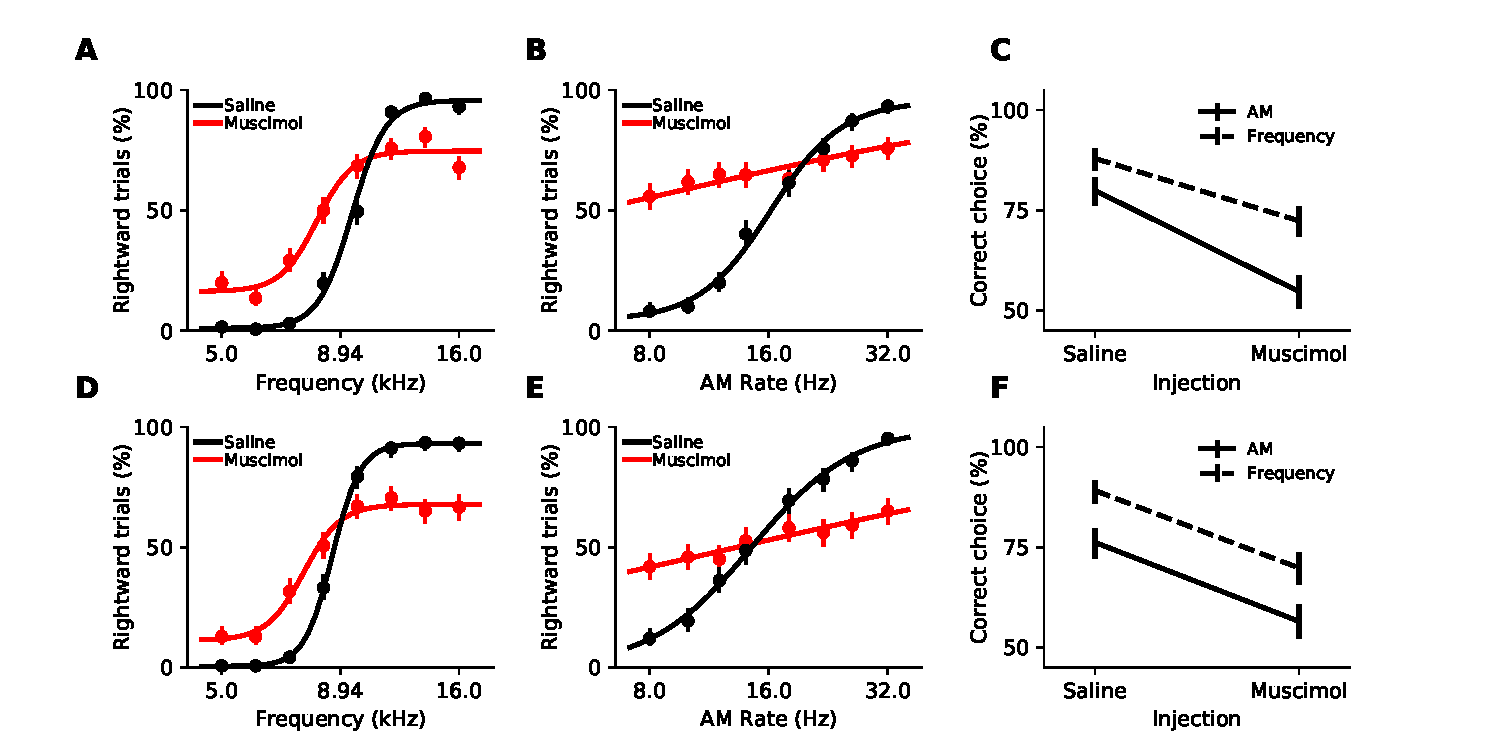
\includegraphics[width=6in]{figures/chapter4/figure_main_amod_effect}%
\end{center} \caption{Reversible inactivation of AC impairs both frequency and
AM discrimination.}{ \textbf{(A)} Frequency discrimination psychometric
performance for subject 1, averaged over 5 saline sessions (black points) and 5
muscimol sessions (red points).
%
\textbf{(B)} AM discrimination psychometric performance for subject 1, averaged
over 5 saline sessions (black points) and 5 muscimol sessions (red points). 
%
\textbf{(C)} Average percent correct for subject 1, averaged over 5 saline
sessions and 5 muscimol sessions.
%
Dotted line indicates the effect of muscimol injection on sound frequency
discrimination performance. 
%
Solid line indicates the effect of muscimol injection on AM rate discrimination
performance.
%
Error bars indicate 95\% binomial proportion confidence intervals.
%
\textbf{(D, E, F)} Same as A, B, and C, respectively, for subject 2.  }
\end{figure}

% The effect of inactivation is not different between the two stimuli (GLMER
% results).

\subsection{AC inactivation affects discrimination of both features when during
sessions with a single sound type}
% DONE: Did they learn both, and then get transferred to 2? Was it the same
% between?
For a subset of animals, we performed reversible inactivation of AC during
sessions where subjects only had to discriminate a single sound type.
%
Under these conditions, we still observed an effect of muscimol both on
psychometric performance (\textbf{\fig{\SinglePsy}}) and on overall percent
correct (\textbf{\fig{\SingleSum}}).

% We have a few sessions where we show that both discriminations are hurt
% individually, arguing against the idea that the cortically-dependent part of
% the task is the switching. 

%%%%%%%%%%%%%%%%%%%%%%%% Figure Single Sound Type %%%%%%%%%%%%%%%%%%%%%%%%%%%%%
\begin{figure}[hp] \begin{center}
	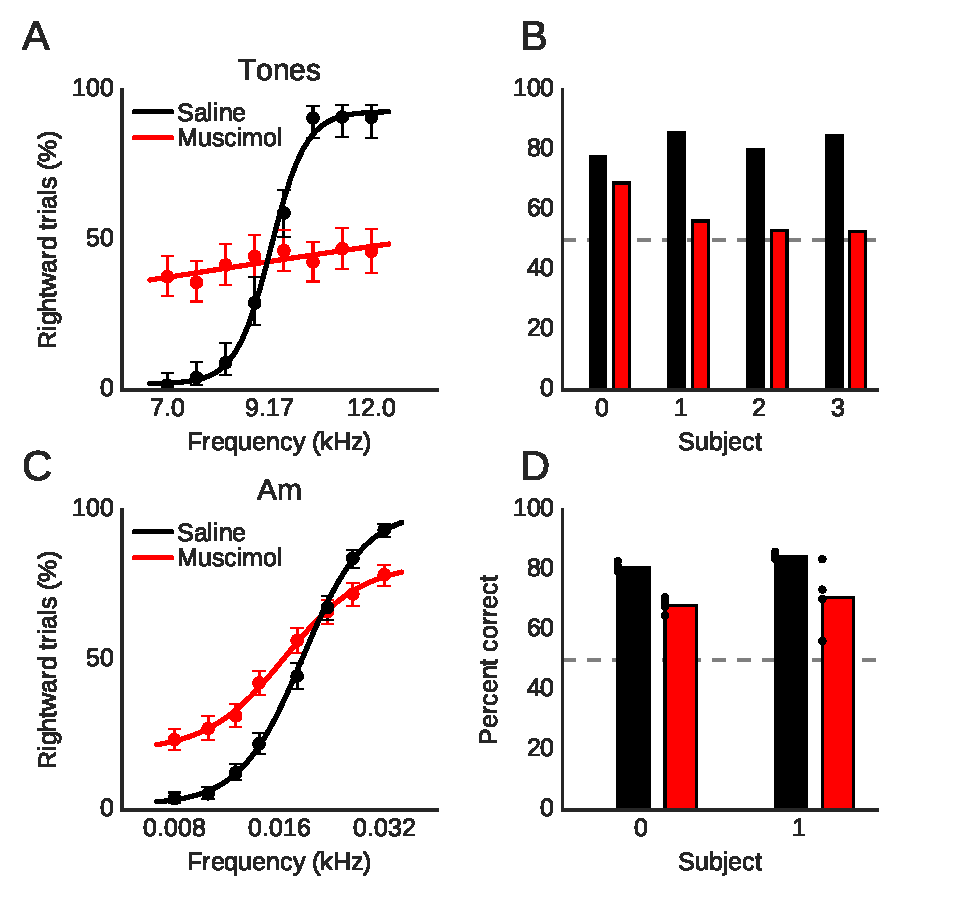
\includegraphics[width=6in]{figures/chapter4/figure_single_sound_type}%
\end{center} \caption{Muscimol affects each discrimination when performed
independently.}{\textbf{(A)}  Example psychometric curve from sessions where an
animal discriminated only high sound frequency from low sound frequency.
Performance suffers in sessions where muscimol was injected in AC (red, 1
session) compared to control saline injection (black, 1 session).
% DONE: How to have number of sessions here? 
%
\textbf{(B)} Average percent correct for 4 animals during muscimol (red, 1
session per animal) and saline (black, 1 session per animal) sessions. 
%
\textbf{(C)} Example psychometric curve from sessions where an animal
discriminated only fast AM rates from slow AM rates. Performance suffers in
sessions where muscimol was injected in AC (red, 4 sessions) compared to
control saline injection (black, 4 sessions).
%
\textbf{(D)} Average percent correct for 2 animals during muscimol (red, 4
sessions per animal) and saline (black, 4 sessions per animal) sessions.  }
\end{figure}


\section{Discussion}

This behavioral paradigm was designed to facilitate comparison of the same manipulation of neural activity on discrimination of two different sound features, in order to address the question: Is auditory cortex required for discrimination of some sound features, while discrimination of other sound features can be accomplished with subcortical pathways alone? 
%
We found that animals were able to learn the task, although it took a long time to train them to perform it at a high degree of accuracy. 
%
We performed reversible inactivation of auditory cortex in two animals trained in this task, and observed deficits in both frequency and AM discrimination. 
%
Future experiments must leverage the flexibility of the 2AFC paradigm, by manipulating the stimulus sets presented, to bring the psychometric performance for each sound type to the same starting point before performing inactivations. 
%
Importantly, we chose to use reversible inactivation with muscimol in this study for several reasons, but this behavioral paradigm can generalize to other inactivation techniques as well. 
%
It is likely that a full picture of the role of sensory cortex in the two discriminations tested would rely on information gained from inactivation experiments with different methods of manipulating or silencing activity. 

\subsection{What about using lesions instead?}
% What is the role of chemical inactivations when you could just do lesions so that you know the exact boundary of the removed tissue?
Lesions have the advantage of allowing precise histological determination of the regions that are removed or damaged. 
%
% TODO : Refs
Lesions can also lead to different results than transient inactivations, an effect often assumed to be related to compensatory plasticity occurring after the lesion and before the behavioral assessment. 
%
However, the comparison of both lesion and transient inactivation experiments can lead to a fuller picture of the role of a brain area in a behavior. 
%
If a downstream region receives connections from both a cortical and a subcortical area, then transient inactivation of the cortical region could lead to unbalanced inputs in the downstream region and cause task deficits, even if the cortical representation of the information isn't any more useful for solving the behavioral task than the subcortical representations. 
%
Following a lesion of the cortical region, the downstream area could undergo homeostatic rebalancing of its inputs, and the discrimination could be solved again using only the input from the subcortical pathway. 
%
In this situation, the lesion study alone may lead to the erroneous conclusion that the cortical region is not at all involved in task performance under normal circumstances, and the transient inactivation experiment would lead to the erroneous conclusion that the information from the subcortical pathway is not sufficient, or at least less useful, for solving the discrimination task. 
%%%%%%%%

%%%%%%%%
A more nuanced way of examining the role of brain regions is laid out in \citet{Otchy2015}. 
%
The authors argue that brain areas should be categorized as \emph{necessary} or \emph{permissive} for task performance by using a combination of both lesion and transient inactivation experiments. 
%
An area is \emph{permissive} for task performance if it is involved in task performance under normal conditions, but doesn't provide any information that can't be obtained from other pathways or areas. 
%
Transient inactivation of a permissive structure will cause deficits in task performance, but lesion of the area, with a recovery period afterward to allow downstream areas to adapt to changes in their inputs, would not.
%
An area that is truly \emph{necessary} provides information that cannot be obtained from another source. 
%
Thus, performance would still suffer after lesion, even if you allow a period for downstream circuits to adapt.

\subsection{What about using optogenetics instead?} % With opto you can use the same fiber over many sessions to standardize the location of the light delivery. 
In the experiments presented here, we chose to perform transient inactivation using muscimol instead of using optogenetic methods. 
%
While optogenetic methods are unparalleled in their ability to allow circuit manipulations with fine temporal resolution, we preferred to use chemical inactivation in this case because we were interested in silencing cortex for the duration of the behavioral session. 
% TODO: Do I want to finish this? 
% If you leave the light on you can burn the brain 
% Also, not all opsins can follow for long periods of time. 
% Most experiments use pulses of light to get around this, but this leads to the potential for local circuit interactions which can cause network activity to do unpredictable things. 

% 2. Fast time-scale manipulations can cause local network effects and mess with
% feedback inhibition and excitation, potentially messing everything up.
% %
% Chemical inactivations allow the brain area to reach a new steady-state that
% will persist for roughly the length of time that the animal is performing the
% behavior.
% %
% It might be possible to leave the light on if using cheeta or some other opsin
% that doesn't get weaker over time, but you run the risk of frying the brain.
% %
% Chemical inactivations don't have that issue. 


\subsection{What did we learn from preliminary inactivations?}
% Need to performance match
% There is an effect on both, so it does make sense to compare the relative strength of inactivations rather than expect that a manipulation will affect one thing but not another. 
We performed inactivations over many behavioral sessions in two trained animals, showing that this method allows us to resolve the effect of the manipulations on discrimination of each sound type. 
%
There are obvious next steps that should be addressed in any experiment going forward. 
%
First and foremost, the performance of animals on the psychometric categorizations for each sound type must be manipulated, by changing the range of stimuli presented, so that performance on the two discriminations is matched before manipulating cortical activity. 
%
If pre-inactivation performance is the same on both sound types, then it becomes much easier to compare the changes in task performance for each sound type. 
%
For our preliminary inactivations, it was not clear whether a decrease from 85\% correct to 75\% correct and decrease from 75\% correct to 65\% correct were effects of equivalent magnitude. 
% TODO: We attempted to address this by doing GLMER regression, talk about that here? 


\section{Link to Chapter V}
In this chapter, we present a behavioral task for evaluating the effect of chemical inactivation of auditory cortex on frequency and AM rate discrimination performance. 
%
% TODO: Change this to highlight the results less. 
We found that inactivation of auditory cortex resulted in reduction in performance for both types of discriminations, with similar (and not statistically significantly different) effect magnitude. 
%
In the next chapter, we expand from considering just the role of auditory cortex in the context of this task, to examine the role of other sensory cortical regions in different tasks requiring animals to make flexible associations between stimuli and actions. 












%%%%%%%%%%%%%%%%%%%%% Old stuff below %%%%%%%%%%%%%%%%%


% 
% 
% 
% 
% This behavioral paradigm solves several problems: 
% %
% Comparing two groups of animals means that you need to be able to correlate the size of each lesion / inactivation with the resulting behavioral deficits observed in each animal. 
% %
% For lesions this is more feasible, but for multiple sessions with reversible inactivation or optogenetic manipulations, this is not feasible. 
% %
% 
% Having animals switch between tasks begins to allow for comparison of manipulations across sound types, although there are still a number of issues. 
% %
% Having an animal switch between sound types after a number of sessions would complicate any comparison because the 
% 
% 
% This behavioral paradigm allows comparison of the same manipulation on 
% 
% 
% 
% 
% 
% In this chapter, I present a behavioral paradigm that can be used to evaluate
% the effects of reversible chemical inactivation of a brain area on
% discrimination of different stimuli. 
% %
% Using this paradigm, I trained mice to perform discriminations both of sound
% frequency and of AM rate.
% %
% Reversible inactivation of AC with muscimol in animals trained on this task
% caused deficits in discrimination of both stimuli. 
% %
% % It looks like the muscimol inactivation affects performance of both tasks to
% % a similar degree. Several possible reasons for this: DONE: This is a bad
% % sentence.
% There are several possible explanations for these results. 
% 
% % TODO: I think there is a better way to go about this. Instead of focusing hard on the results of the inactivations (which are really preliminary with only two mice) I should talk more about the behavior here and why we need something like this.
% %
% % TODO: Then use the inactivation data to highlight some of the analysis concerns (like the need to performance match).
% %
% % TODO: This avoids the necessity to really go after the comparison to the lesion studies (which aren't super clear anyway) and simply explain why the data is tough to analyze and what can be done about it.
% 
% %%%%% Analysis considerations %%%%%
% % Have to performance match, because it's hard to compare across the performance space. 
% % Fluorescent muscimol, optogenetics, or lesions? How to combine them for best information? 
% 
% 
% 
% 
% %
% % TODO: I should probably remove the figure about the single sound types. 
% 
% 
% % TODO: Better title here
% \subsection{Why did we see effects of muscimol on both frequency and AM
% discrimination?}
% 
% The effect of reversible inactivation of AC on frequency discrimination we observed in this pilot was somewhat stronger than the relatively minor frequency discrimination performance observed in rats after nearly complete lesions of AC in \citet{Gimenez2015}.
% % Mice vs. Rats
% This may be due to differences in the relative contribution of auditory cortex to frequency discrimination between these two species. 
% % Don't know if muscimol is spreading farther
% Also, muscimol may be spreading to inactivate cortical or subcortical areas outside the areas lesioned in \citet{Gimenez2015}.
% % Cortical dependence due to switching
% There is also the chance that auditory cortex is more involved in the performance of this task due to the switching involved.
% % Permissive vs. Necessary with reversible inactivations.
% Lastly, it is possible that the effect of sudden, reversible inactivation of AC overestimates this area's necessity because it leads to transient unbalancing in downstream areas that could, if given enough time, undergo homeostatic rebalancing. 
% 
% % TODO: Need to make sure I talk about what has to be improved for the future (ideally use fluorescent muscimol to track where it goes and performance match pre-muscimol by messing with the stimulus range.)
% 
% % TODO: Write better words
% %% Downstream circuits are expecting input from AC, and don't have time to complete the homeostatic rebalancing necessary to make use of information from a single source.
% One reason has to do with the necessary/permissive nature of the relationship
% between a brain area and a behavior \citep{Otchy2015}.
% %% Less likely that the task switching component is adding an additional layer of cortical dependence, as inactivation of AC before performance of either task alone leads to performance deficits. 
% An alternative explanation is that the switching component of the task
% introduced an additional process that depends on the cortex, outside of the
% individual sound-action associations. 
% %%% Subcortical circuits can accomplish significant flexibility on a short time scale (Gimenez paper) but this is switching every trial
% However, I believe that this is less likely for three reasons.
% 
% First, rodents have been shown to be capable of remarkable levels of
% flexibility after nearly-complete removal of auditory cortex, switching the
% action associated with a particular sound several times during a single
% behavioral session \citep{Gimenez2015}.
% %
% %%% During training, animals learn each association independently (which takes the most time) and then learn to switch between them, which takes little time TODO: Plot this.
% Second, animals took longest during the training steps in which they were
% learning the individual sound-action associations, and took few trials to
% achieve a high degree of accuracy after they started having to switch between
% sound types in the same behavior session.
% %%% Deficits caused by cortical inactivation also appear during individual AM or freq discrimination sessions, so not all effect can be related to switching. 
% Lastly, we tested the effect of reversible AC inactivation during sessions with
% only a single sound type in a subset of animals.
% % TODO: I have to figure out why the effect of muscimol on frequency discrimination is so strong in the session's I've plotted. It's concerning.
% %
% We observed deficits in discrimination performance during sessions with only
% tonal stimuli and during sessions with just AM stimuli, suggesting that the
% sound-action associations themselves are impacted by cortical inactivation.
% %
% Nonetheless, it is worth evaluating whether the additional complexity
% introduced by switching between sound types every other trial is really
% required to answer our main question. 
% 
% \subsection{Why use this method if the switching might complicate things?}
% 
% % This method took a long time to learn and there is a chance that the
% % switching component introduced additional complexity.
% %
% % So do we need to use the task? Why is this better than the alternatives? 
% This task required mice to learn two different sound-action associations, and
% then to switch back and forth between them every other trial of a behavior
% session.
% %
% Though this method presents the obvious drawbacks of taking a long time to
% learn and potentially engaging additional brain areas to mediate the switching,
% it allows us to evaluate the effect of a single manipulation of brain activity
% on both discrimination behaviors, which is critical to addressing our main
% question.
% 
% % Attempts to evaluate the effect of reversible inactivations on several
% % different discriminations are hampered by the time course of the
% % inactivation, and the fact that a bolus delivered on one day may not reach
% % the exact same tissue area as a bolus delivered the next day.
% Attempts to compare the effect of inactivations on task performance in two
% different groups of animals performing the same task would invariably be
% hampered by the inability to tell precisely the extent and strength of the
% inactivation across individuals.
% %
% Even optogenetics, as will be discussed below, cannot fully address this
% problem, especially if we desire to compare the size of the effect on the two
% different task types.
% 
% % Problems addressed by this method:
% 
% %% Hard to compare relative effects of inactivations on different tasks across animals (one task per animal)
% %%% Lesions: Have to compare lesion area across animals
% %%% Muscimol: Have to compare bolus between animals, which may be impossible (except maybe with fluorescent muscimol).
% %%% Optogenetics: Have to try and compare inactivated area between animals, which may be impossible. TODO: Paper Ben K presented about photobleaching relevant here.
% 
% %% Many problems still persist if you have an animal perform both tasks, but not on the same day
% %%% Lesions: Time course of homeostatic rebalancing may interfere if different tasks are performed sequentially over days
% %%% Muscimol: A bolus one day is not directly equivalent to a bolus the next, and fluorescent muscimol can't help you at all with that. 
% %%% Optogenetics: This is less of an issue for opto, where the effects of the laser should be roughly consistent from day to day. TODO: Anything about glia growth around fibers?
% 
% %% Having animals perform both tasks during the same behavior session addresses some of these sources of variation.
% %%% Lesions: Circuit rebalancing should be occurring at roughly the same pace and affecting both discriminations across assessment days.
% %%% Muscimol: The effect of a single bolus can be evaluated on both tasks.
% %%% Optogenetics: The state of the fiber, tether, diode, etc that may vary from session to session are more controlled across the two tasks. 
% 
% \subsection{Are chemical inactivations useful in a world with optogenetics?}
% % This is still an open question in my mind.
% 
% % TODO: Why use muscimol at all?? The problem that we are addressing with this
% % interleaved task is that the inactivation wears off. This isn't as much of a
% % problem with lesions, although there is still the possibility that downstream
% % circuits are adapting to the changes, and so sampling different tasks on
% % different days could still be a problem.
% 
% % Comparisons of lesions and optogenetics TODO: There is a paper doing visual
% % cortex opto that argues against lesions.
% %% Lesions: Allow time for downstream circuits to rebalance their inputs, potentially underestimating the contribution of other pathways.
% %% Optogenetics: Near-instantaneous inactivation provides no chance for downstream circuits to rebalance, potentially overestimating the contribution of an area.
% %% Muscimol: The worst of both worlds or better than both? Muscimol is like CNO (TODO: check arguments for CNO) but affects everything, not just HM4+ neurons, and may be stronger than HM4 inactivation (TODO: Check HM4 vs muscimol inactivation strength). Also, there is some evidence that CNO decomposes to clozapine and becomes active elsewhere besides just at the HM4 receptors (TODO: Check new CNO to clozapine study).
% 
% % TODO: Future improvements to the task include better initial performance
% % matching
% 
% Lesion studies have long been the gold standard method for evaluating the
% %
% A potential confound of lesions studies is often discussed: That during the
% time after the lesion, subcortical pathways reorganize to carry out the
% function that was previously provided by the cortex.
% %
% This confound rightly prevents us from inferring that cortex \emph{does not}
% play a role in some particular task, if it is found that an animal is able to
% perform the task after a lesion of the cortex.
% %
% However, with emerging anatomical studies showing extensive convergence of
% cortical and thalamic pathways onto structures like the striatum
% \citep{Hunnicutt2016} it is likely that both the cortical and subcortical
% pathways are providing information to downstream regions during normal
% conditions.
% %
% The re-organization of subcortical pathways following cortical lesion could
% simply be a homeostatic rebalancing of already-existing connections between the
% subcortical pathway neurons and the downstream region.
% %
% In this context, we should interpret the persistence of a behavior after
% cortical lesion to mean that the cortex wasn't providing necessary information
% for that behavior, not that it wasn't involved at all.
% 
% % TODO: Cite Otchy and whatever paper was doing orientation change detection
% % suppression in rats (Glickfeld and Maunsell)
% Studies have repeatedly shown that fast, reversible inactivations (such as
% those achieved with muscimol or various optogenetic methods) can lead to
% different effects on the same behavior than are caused by lesions. 
% %
% % TODO: Getting harder to write here. Come back to this. 
% 
% Chemical inactivations complement lesions in the sense that they allow you to
% test whether an area is providing information to downstream circuits under
% normal conditions.
% %
% % TODO: this is shit and needs citations
% Optogenetics is fancy and all, but has a few problems.
% %
% 1: You can't really leave the light on forever and expect things to work as
% planned.
% %
% 2. Fast time-scale manipulations can cause local network effects and mess with
% feedback inhibition and excitation, potentially messing everything up.
% %
% Chemical inactivations allow the brain area to reach a new steady-state that
% will persist for roughly the length of time that the animal is performing the
% behavior.
% %
% It might be possible to leave the light on if using cheeta or some other opsin
% that doesn't get weaker over time, but you run the risk of frying the brain.
% %
% Chemical inactivations don't have that issue. 
% 
% % TODO: 
% We should combine this task with rigorous combinations of transient inactivation and lesion studies to determine whether regions are truly necessary for task performance, or if they are permissive for task performance, in the sense that downstream areas receive connections and therefore transient inactivation will lead to unbalanced inputs that could be homeostatically rebalanced over time
% 
